\documentclass[10pt]{beamer}
\usetheme[progressbar=frametitle]{metropolis}
\usepackage{appendixnumberbeamer}
\usepackage{booktabs}
\usepackage[scale=2]{ccicons}
% \usepackage[ngerman]{babel}
\usepackage{graphicx} 
% \graphicspath{ {images/}  {../images/} }
\usepackage{tikz} 
\usepackage{wrapfig}
%\usepackage[utf8]{inputenc}
%\usepackage[T1]{fontenc}
\usepackage{moreverb}
\usepackage[backend=biber]{biblatex}   
\addbibresource{content/cites.bib}
%\bibliography{content/cites.bib}
\usepackage{textcomp}
%\usepackage{fontspec}
%\setsansfont{Fira Sans}
\usepackage{hyperref}
\usepackage{animate}
\renewcommand*{\bibfont}{\scriptsize}
%\usepackage{caption}
%\captionsetup[figure]{labelformat=empty}% redefines the caption setup of the figures environment in the beamer class.

\title{Mid-term Presentation}
\author{András Czuczi, Samy Dafir, Andreas Lindlbauer} %#nohomo
\date{}
\begin{document}

\begin{frame}
	\maketitle 
\end{frame}

%%%%%%%%%%%%%%%%%%%%%%%%%%%%%%%%%%%%%%%%%%%%%%%%%%%%%%%%%%%%%%%%%%%%%%%%%%%%%%%%%%%%%%%%%%%%%%%%

\begin{frame}{Overview}
	\tableofcontents
\end{frame}

%%%%%%%%%%%%%%%%%%%%%%%%%%%%%%%%%%%%%%%%%%%%%%%%%%%%%%%%%%%%%%%%%%%%%%%%%%%%%%%%%%%%%%%%%%%%%%%%

\section{Summary of subnetTALK}

%%%%%%%%%%%%%%%%%%%%%%%%%%%%%%%%%%%%%%%%%%%%%%%%%%%%%%%%%%%%%%%%%%%%%%%%%%%%%%%%%%%%%%%%%%%%%%%%

\begin{frame}{Human Building Interaction by Selena Savić I.} 
	\begin{itemize}
        \pause{}
		\item Human Building Interaction (HBI) focuses on resources and therefore on budgeting
		\pause{}
		\item Goal is to end the talk about whether resources are (in) finite
		\pause{}
		\item Scarcity of resources (whether artificial or not) has an impact on the design
		\pause{}
		\item Just because something is not scarce, no overusage is recommended (eg. WiFi and routers)
	\end{itemize}	
\end{frame}

%%%%%%%%%%%%%%%%%%%%%%%%%%%%%%%%%%%%%%%%%%%%%%%%%%%%%%%%%%%%%%%%%%%%%%%%%%%%%%%%%%%%%%%%%%%%%%%%

\begin{frame}{Human Building Interaction by Selena Savić II.}
	\begin{itemize}
        \pause{}
		\item Computation has an impact on design of buildings -> smart buildings
		\pause{}
		\item Intelligent walls: optimize bandwith usage
		\pause{}
		\item RAM house: a prototype partially made of Radar Absolvent Material -> airplane mode for your house
		\pause{}
		\item Smart home: home expects user to do something (eg.\ use less energy at given time)
	\end{itemize}	
\end{frame}

%%%%%%%%%%%%%%%%%%%%%%%%%%%%%%%%%%%%%%%%%%%%%%%%%%%%%%%%%%%%%%%%%%%%%%%%%%%%%%%%%%%%%%%%%%%%%%%%

\section{Main findings from literature review}

%%%%%%%%%%%%%%%%%%%%%%%%%%%%%%%%%%%%%%%%%%%%%%%%%%%%%%%%%%%%%%%%%%%%%%%%%%%%%%%%%%%%%%%%%%%%%%%%

\begin{frame}{Main findings from literature review I.}
	\metroset{block=fill}
	\begin{block}{Intersection of architecture and interaction design}
	\begin{itemize}
        \pause{}
		\item Interaction with space instead of stuff
        \pause{}
		\item Architectural and spatial metaphors in interfaces
        \pause{}
        \item Technology and architecture (CAD and embedded systems)
        \pause{}
        \item Architectonic technology (e.g\ Media fa\c{c}ades)
	\end{itemize}	
	\end{block}
\end{frame}

%%%%%%%%%%%%%%%%%%%%%%%%%%%%%%%%%%%%%%%%%%%%%%%%%%%%%%%%%%%%%%%%%%%%%%%%%%%%%%%%%%%%%%%%%%%%%%%%

\begin{frame}{Main findings from literature review II.}
    \begin{figure}
    \centering
    \animategraphics[width=300pt,loop,autoplay]{12}{images/frame-}{0}{19}
    \caption{Puzzle Facade by Javier Lloret}
    \end{figure}
\end{frame}

%%%%%%%%%%%%%%%%%%%%%%%%%%%%%%%%%%%%%%%%%%%%%%%%%%%%%%%%%%%%%%%%%%%%%%%%%%%%%%%%%%%%%%%%%%%%%%%%

\begin{frame}{Main findings from literature review III.}
	\metroset{block=fill}
	\begin{block}{Adaptable architecture and feedback loops}
	\begin{itemize}
        \pause{}
		\item More interactive capabilities that have impact
        \pause{}
		\item ``Responsive Places'' change according to occupants needs
        \pause{}
        \item Buildings and their use change over time, allow better appropriation and renovation
        \pause{}
		\item Focus on feedback loop between humans and buildings
	\end{itemize}	
	\end{block}

\end{frame}

%%%%%%%%%%%%%%%%%%%%%%%%%%%%%%%%%%%%%%%%%%%%%%%%%%%%%%%%%%%%%%%%%%%%%%%%%%%%%%%%%%%%%%%%%%%%%%%%

\section{Most interesting findings from SOTA}

%%%%%%%%%%%%%%%%%%%%%%%%%%%%%%%%%%%%%%%%%%%%%%%%%%%%%%%%%%%%%%%%%%%%%%%%%%%%%%%%%%%%%%%%%%%%%%%%

\begin{frame}{SOTA Findings}
	\metroset{block=fill}
	\begin{block}{Main Developments}
	\begin{itemize}
		\item Simplification and Optimisation
		\item Comfort
		\item Privacy
		\item Health
		\item Dynamic Living Spaces
		\item Implicit Interactions
	\end{itemize}	
	\end{block}
\end{frame}


\begin{frame}{SOTA Findings}
	\metroset{block=fill}
	\begin{block}{Main idea behind the smart home}
		\begin{itemize}
		\item Make everyday life easier, more efficient, comfortable and healthier.
		\item Use technology for everything, but keep privacy
		\end{itemize}
	\end{block}

	\begin{exampleblock}{Additional Developments}
	\begin{itemize}
		\item Implicit interactions: Interacting without actually interacting
		\item Adapt to shrinking living space
	\end{itemize}
\end{exampleblock}
	
\end{frame}


\section{Examples / Projects}


\begin{frame}{RAM House}
	\textbf{Dynamic Privacy}\\
	\vspace{3mm}
	\begin{figure}[H]
	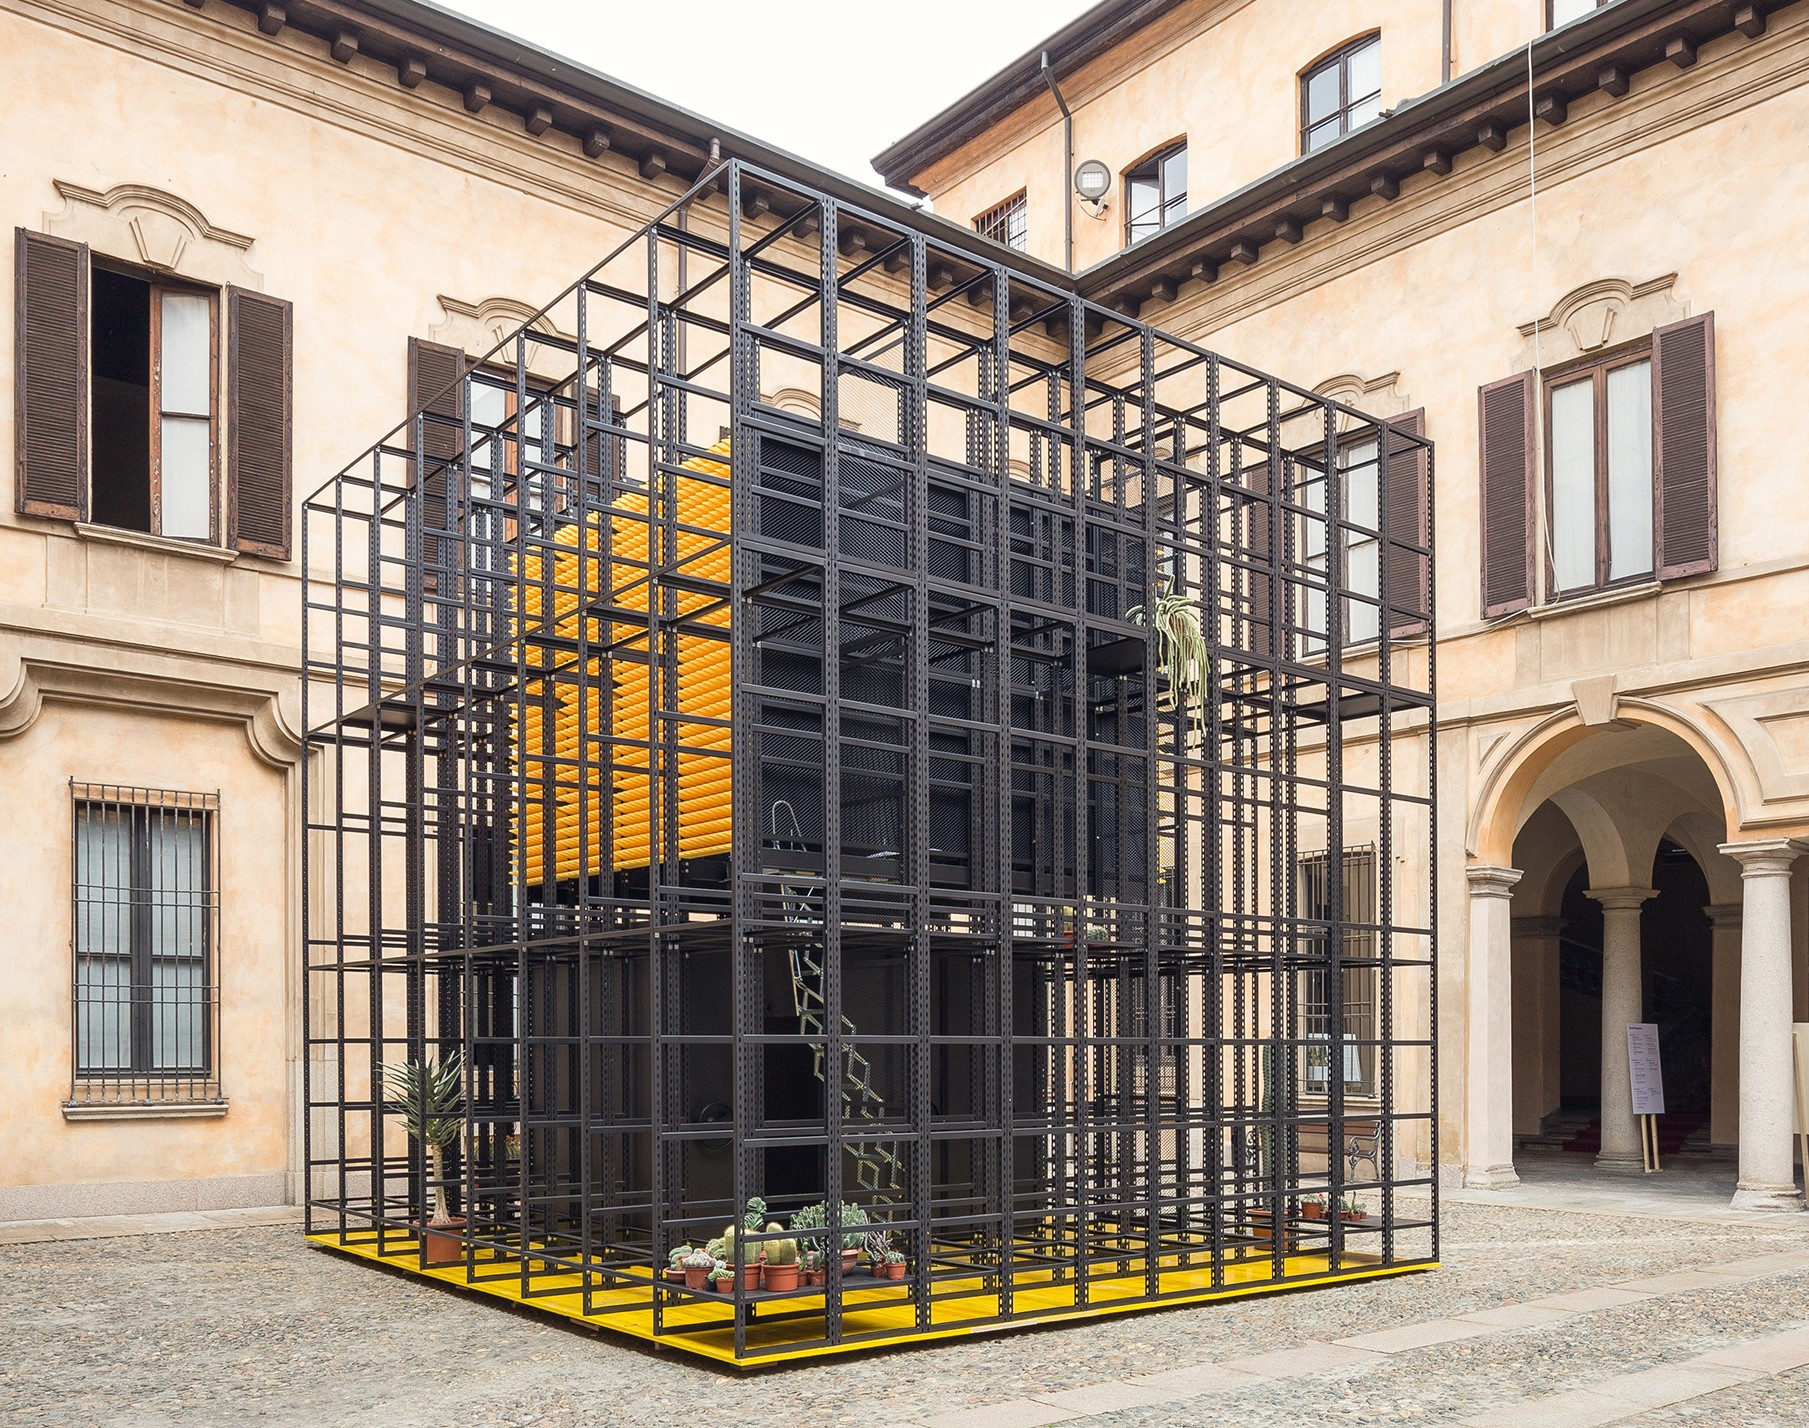
\includegraphics[width=0.7\textwidth]{images/1.jpg}
	\caption{http://www.spacecaviar.net/ram-house/}
	\end{figure}
\end{frame}

\begin{frame}{Numi Toilet}
	\textbf{Comfort and Implicit Interaction}\\
	\vspace{3mm}
	\begin{figure}[H]
	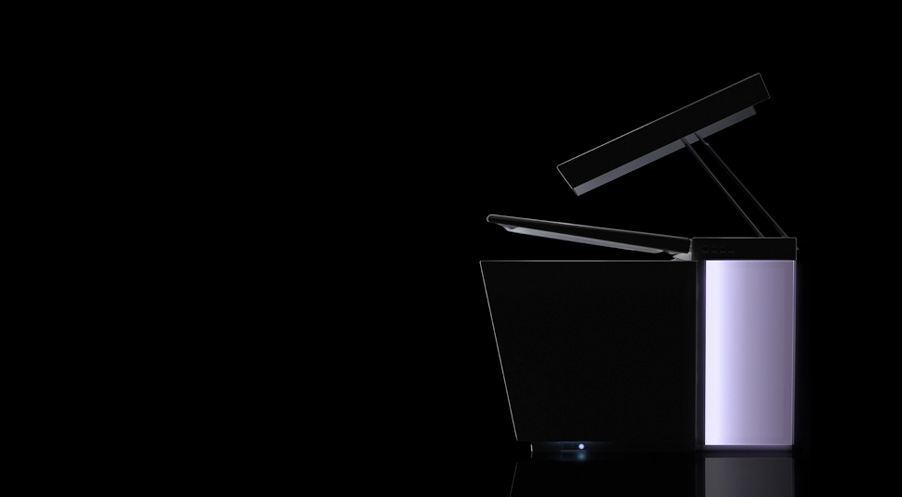
\includegraphics[width=\textwidth]{images/3.jpg}
	\caption{http://www.kohler.com/numi/}
	\end{figure}
\end{frame}

\begin{frame}{Numi Toilet}
	\begin{figure}[H]
	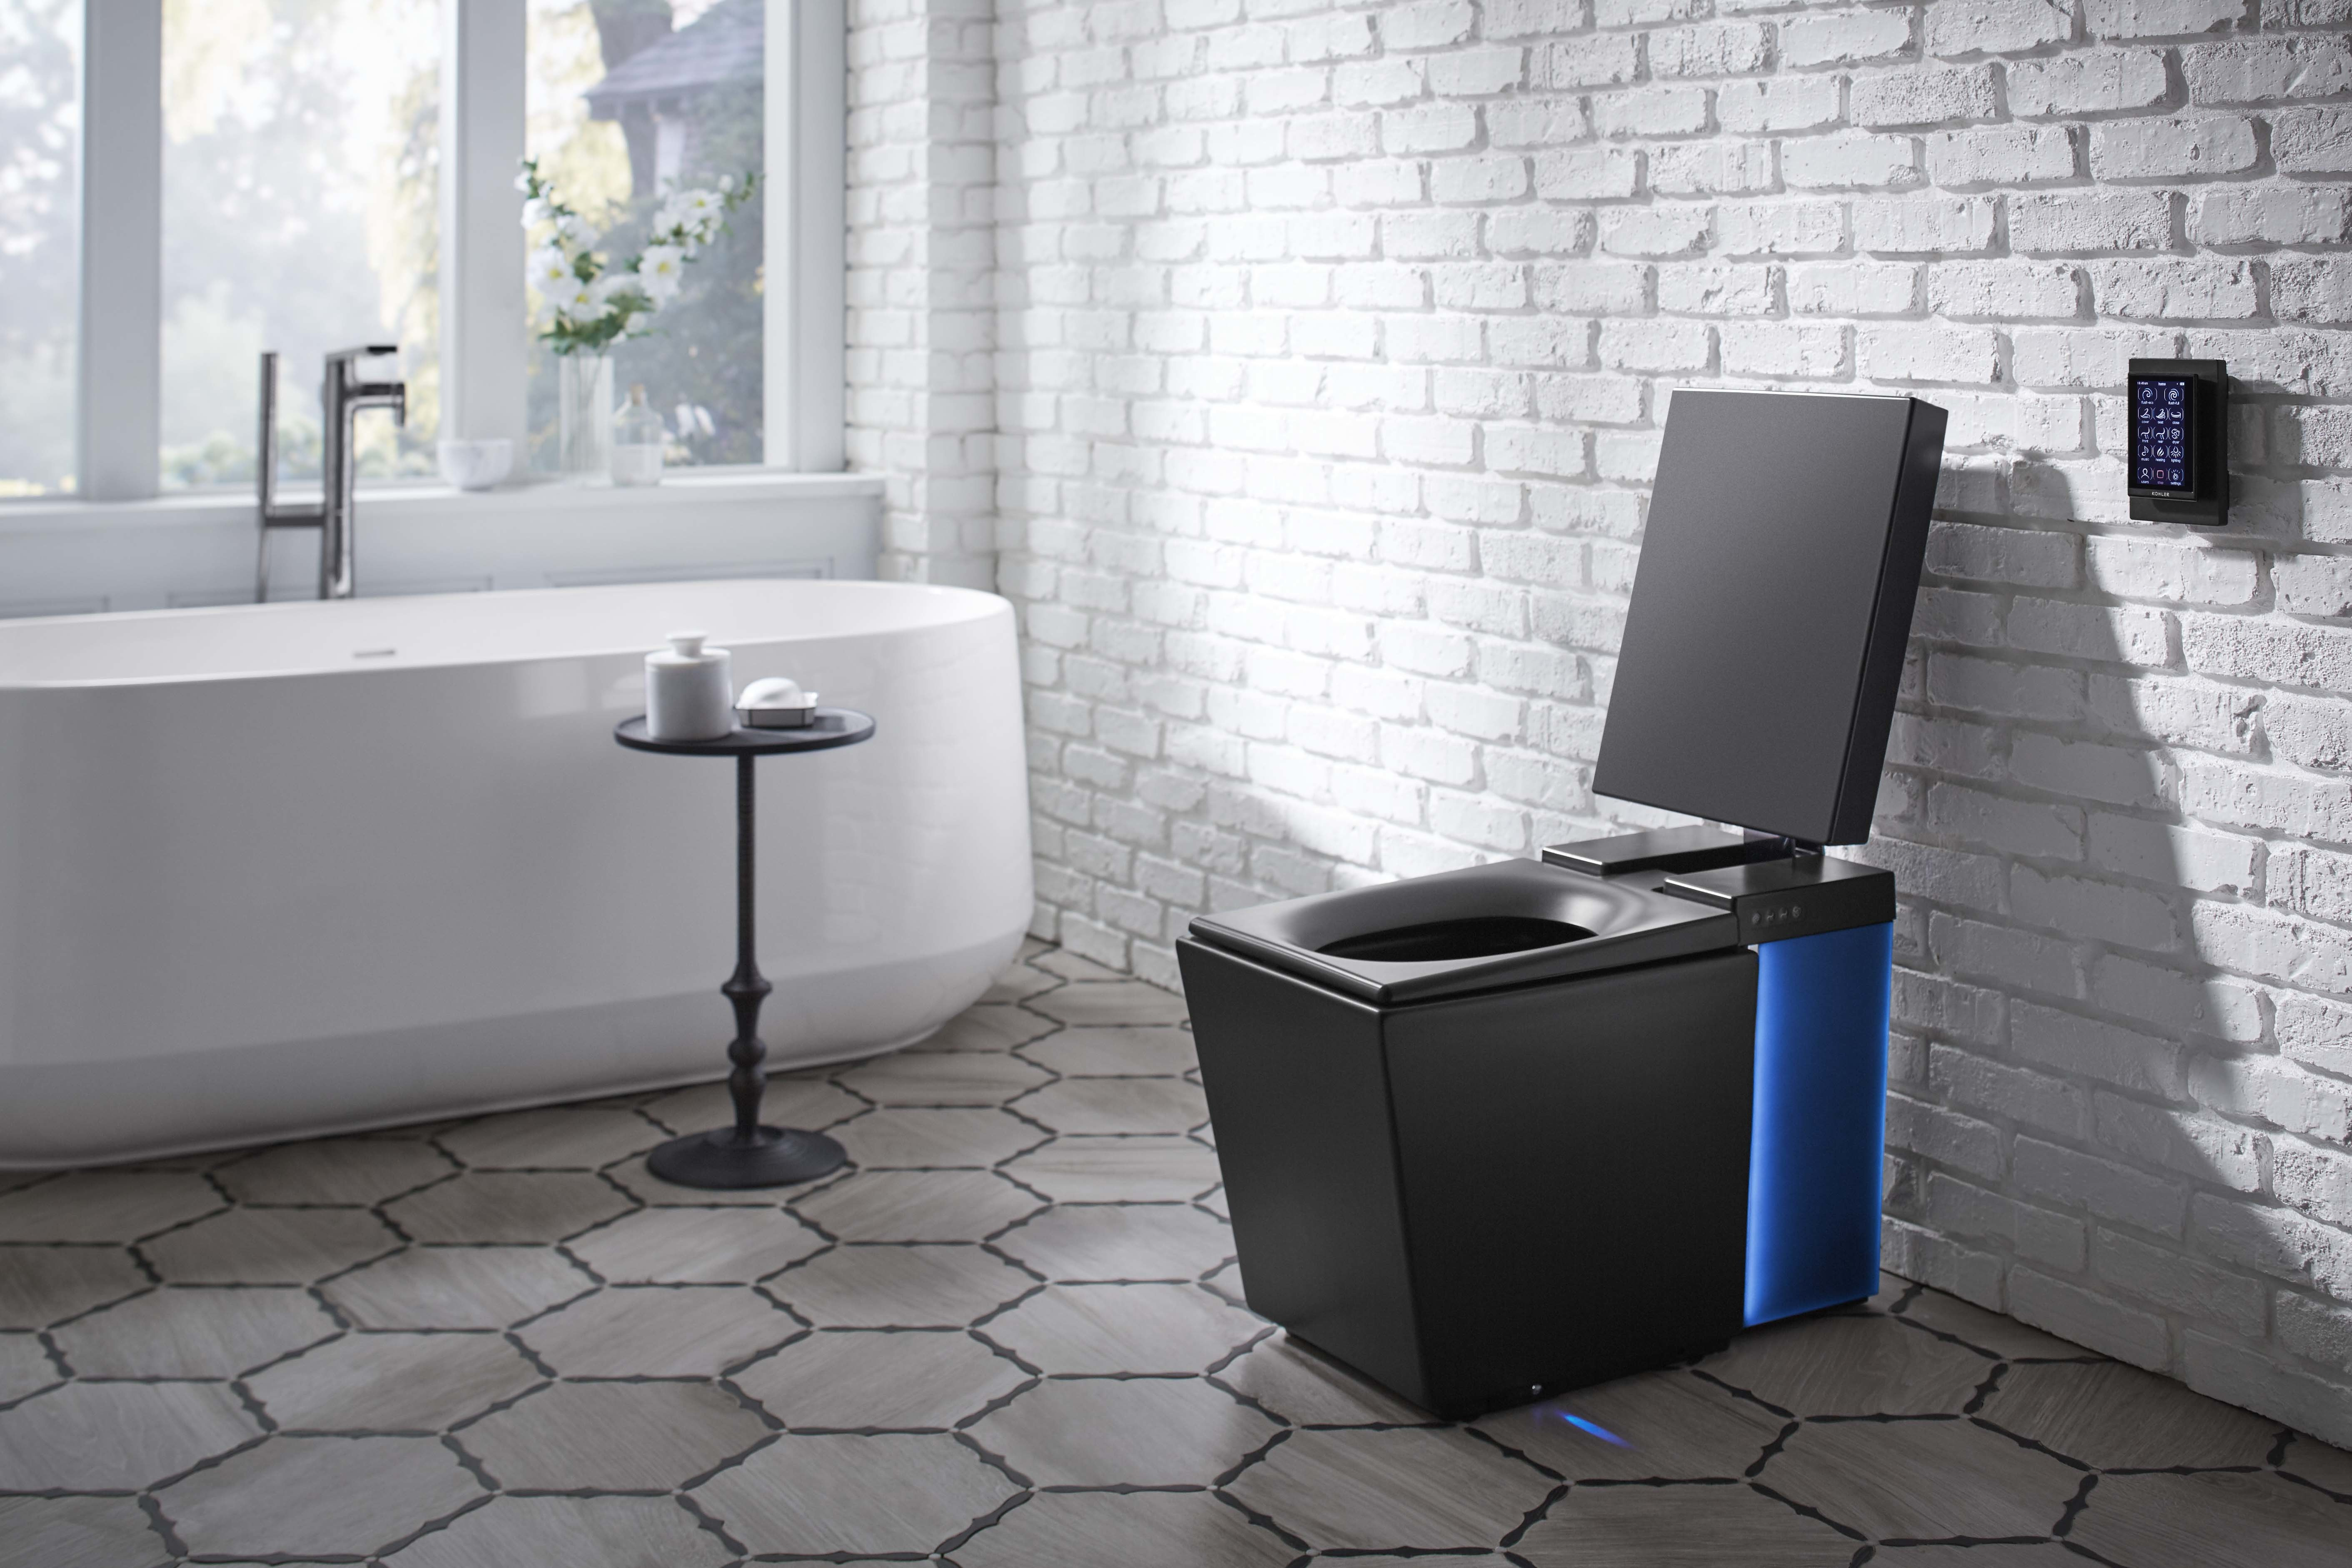
\includegraphics[width=\textwidth]{images/6.jpg}
	\caption{http://www.kohler.com/numi/}
	\end{figure}
\end{frame}

\begin{frame}{MIT CitiHome Project}
	\textbf{Dynamic Living Space}\\
	\vspace{3mm}
	\begin{figure}[H]
	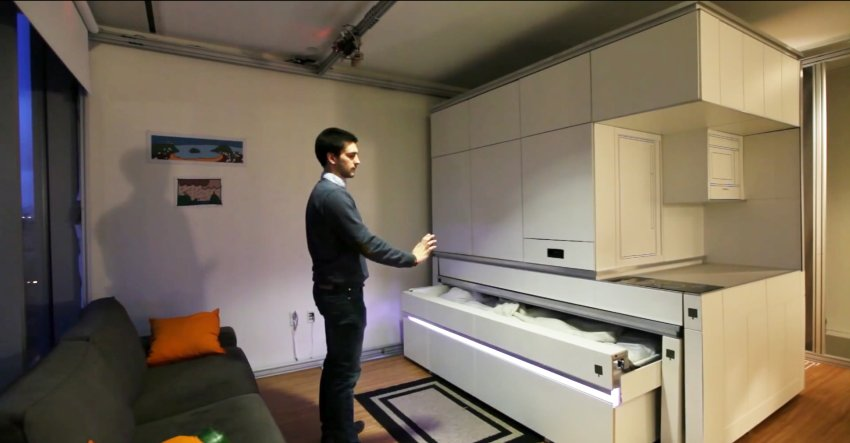
\includegraphics[width=\textwidth]{images/4.jpg}
	\small\caption{https://www.media.mit.edu/projects/OLD\_cityhome2/overview/}
	\end{figure}
\end{frame}

\begin{frame}{MIT CitiHome Project}
	\begin{figure}[H]
	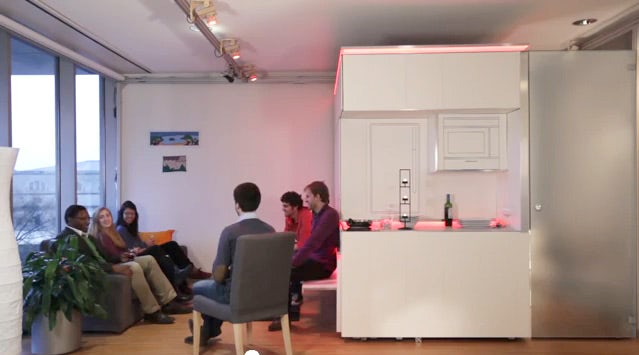
\includegraphics[width=\textwidth]{images/5.jpg}
	\caption{https://www.media.mit.edu/projects/OLD\_cityhome2/overview/}
	\end{figure}
\end{frame}

\begin{frame}{Infrascan Smart Toilet}
	\textbf{Health and Implicit Interaction}\\
	\vspace{3mm}
	\begin{figure}[H]
	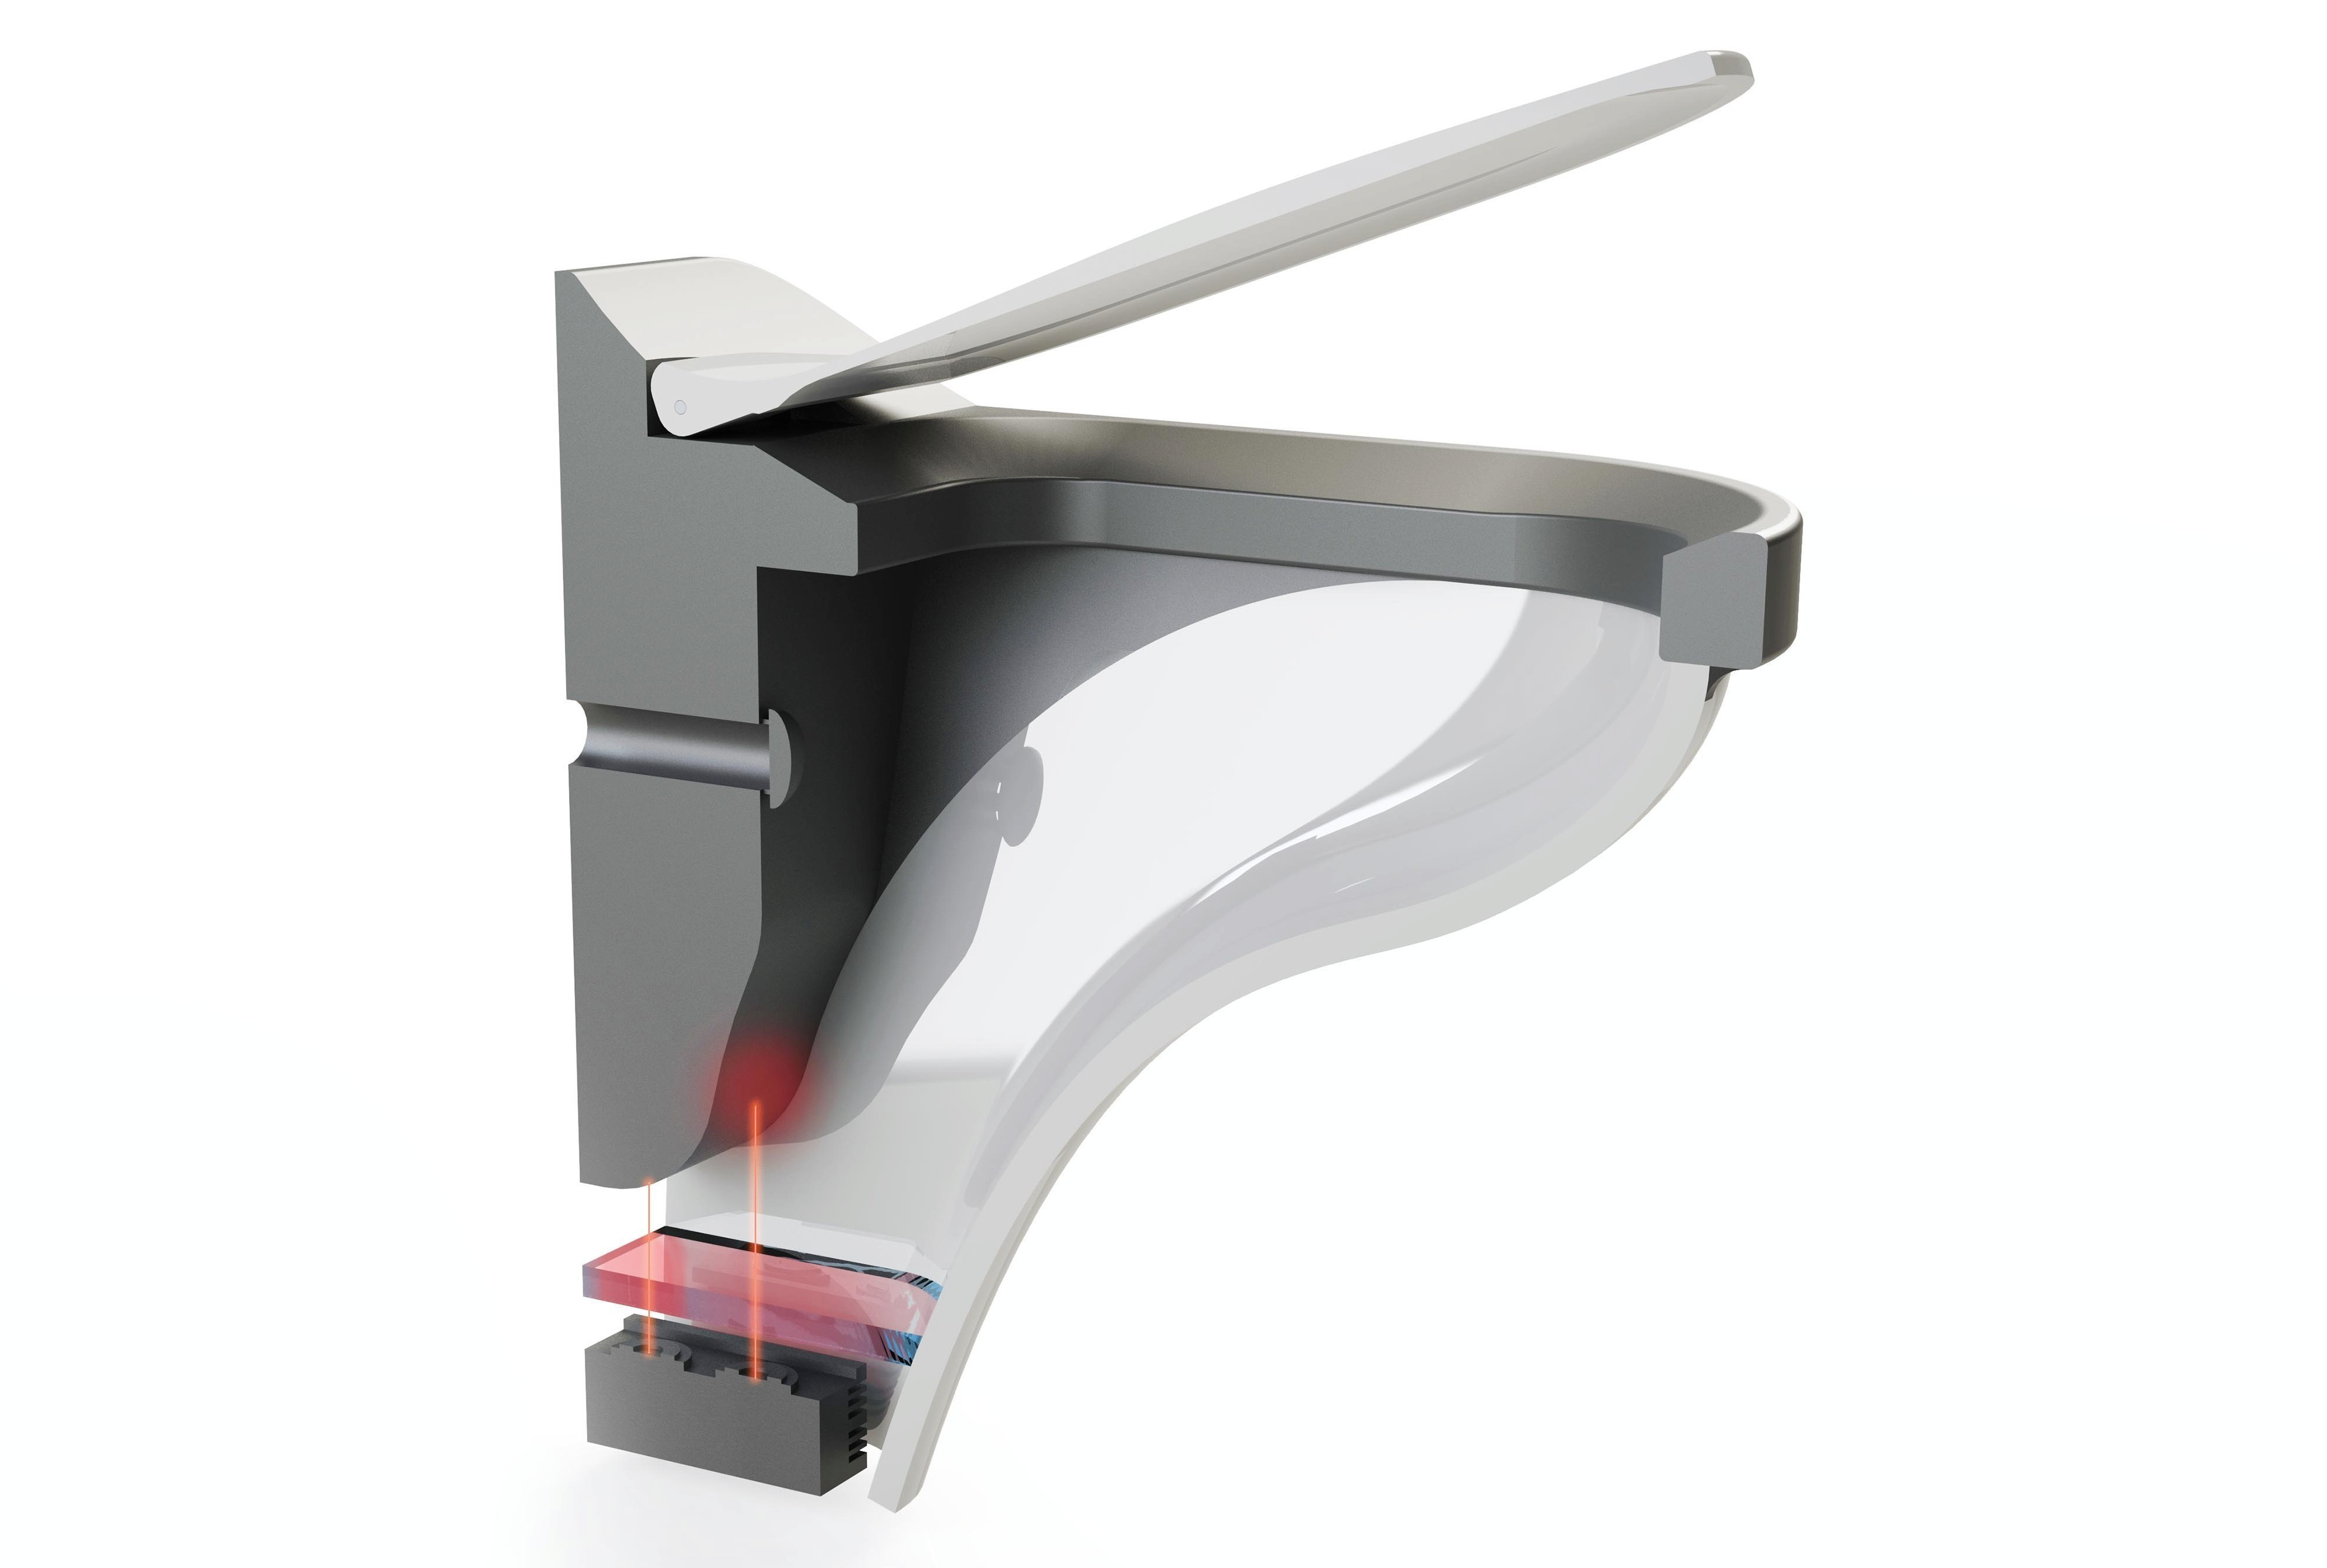
\includegraphics[width=0.8\textwidth]{images/7.png}
	\small\caption{https://www.jamesdysonaward.org/2018/project/infrascan-smart-toilet/}
	\end{figure}
\end{frame}

\begin{frame}{Intellithings RoomMe}
	\textbf{Simplification, Comfort, Implicit Interaction}\\
	\vspace{3mm}
	\begin{figure}[H]
	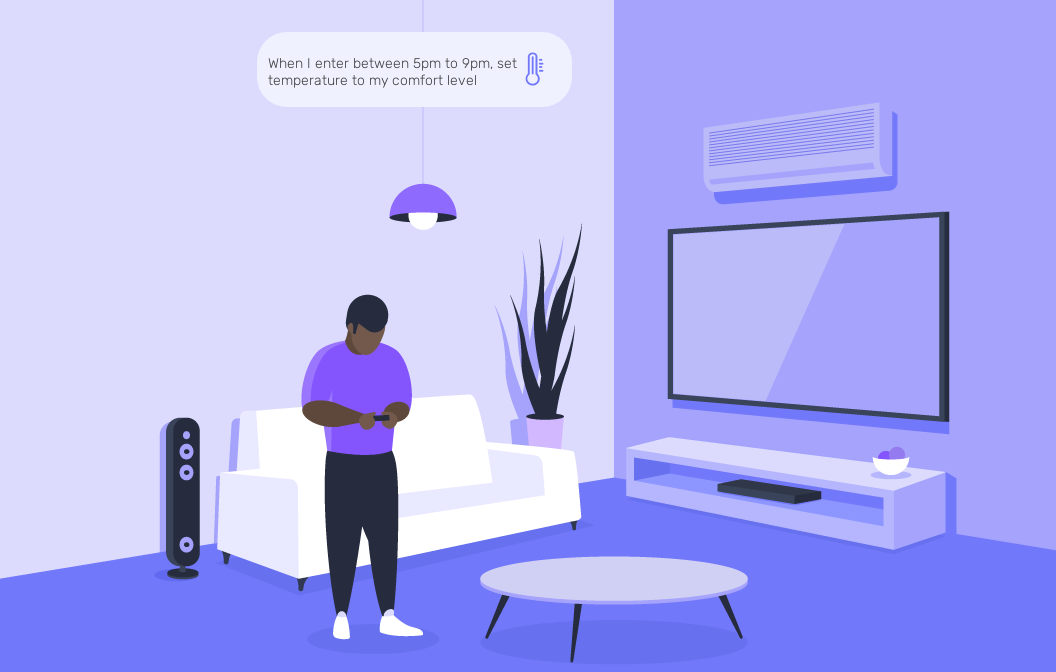
\includegraphics[width=0.9\textwidth]{images/1.png}
	\caption{https://www.intellithings.net}
	\end{figure}
\end{frame}

%%%%%%%%%%%%%%%%%%%%%%%%%%%%%%%%%%%%%%%%%%%%%%%%%%%%%%%%%%%%%%%%%%%%%%%%%%%%%%%%%%%%%%%%%%%%%%%%

\section{Interview Plan}

%%%%%%%%%%%%%%%%%%%%%%%%%%%%%%%%%%%%%%%%%%%%%%%%%%%%%%%%%%%%%%%%%%%%%%%%%%%%%%%%%%%%%%%%%%%%%%%%

\begin{frame}{Experts}
	\begin{itemize}
        \pause{}
		\item Mikael Wiberg Professor of Informatics, Umeå University, Sweden
		\pause{}
		\item Holger Schnädelbach Senior Researcher in the Mixed Reality Lab (MRL), University of Nottingham, GB
		\pause{}
		\item Hamed Alavi Senior Researcher in Human-IST Institute, University of Fribourg, Switzerland
	\end{itemize}	
\end{frame}

%%%%%%%%%%%%%%%%%%%%%%%%%%%%%%%%%%%%%%%%%%%%%%%%%%%%%%%%%%%%%%%%%%%%%%%%%%%%%%%%%%%%%%%%%%%%%%%%

\begin{frame}{Questions I.}
	\begin{itemize}
        \pause{}
		\item How would you define HBI\@? Would you like to change anything about HBI\@?
		\pause{}
		\item What is its relation to HCI and vice-versa?
		\pause{}
		\item Are there HBI-realted projects you are currently working on? Do you plan any? If yes, please elaborate. 
		\pause{}
		\item What was/were the most excited project(s) you took part in?
		\pause{}
		\item What are good and bad examples of HBI\@? Ones you personally had experience with?
	\end{itemize}	
\end{frame}

%%%%%%%%%%%%%%%%%%%%%%%%%%%%%%%%%%%%%%%%%%%%%%%%%%%%%%%%%%%%%%%%%%%%%%%%%%%%%%%%%%%%%%%%%%%%%%%%

\begin{frame}{Questions II.}
	\begin{itemize}
        \pause{}
		\item Is HBI roughly the same around the world? Or are there any significant differences?
		\pause{}
		\item How can HBI used in semi-buildings (eg. boat, camper van)? Or in non-buildings (eg. public transportation vehicles, parks)?
		\pause{}
		\item What do you think about feng-shui?
		\pause{}
		\item Do you support the idea of smart homes? Why (not)?
		\pause{}
    \item When it comes to inventions, many times fiction makes it into reality. Is this the case in HBI, too? Think about literature, films, art and gaming.
	\end{itemize}	
\end{frame}

%%%%%%%%%%%%%%%%%%%%%%%%%%%%%%%%%%%%%%%%%%%%%%%%%%%%%%%%%%%%%%%%%%%%%%%%%%%%%%%%%%%%%%%%%%%%%%%%

\begin{frame}{Questions III.}
	\begin{itemize}
        \pause{}
		\item What kind of interactive architecture design element would you like to see in [town of his university] (even aside reality)?
		\pause{}
    \item How could have you used your knowledge about HBI from nowadays for example in mediaval times? Eg. on a simple home and on a castle.
		\pause{}
		\item Imagine the idea of constructing a hotel full of rooms which (almost futuristically) adapt to their guests and their mood (like the mood ring or music playing based on mood, etc). Is such thing possible? If yes, how?
		\pause{}
		\item What development do you expect for the near future (\~{}10 years)? And in the next \~{}50 years?
	\end{itemize}	
\end{frame}

%%%%%%%%%%%%%%%%%%%%%%%%%%%%%%%%%%%%%%%%%%%%%%%%%%%%%%%%%%%%%%%%%%%%%%%%%%%%%%%%%%%%%%%%%%%%%%%%
	%{\footnotesize \printbibliography}
  

%%%%%%%%%%%%%%%%%%%%%%%%%%%%%%%%%%%%%%%%%%%%%%%%%%%%%%%%%%%%%%%%%%%%%%%%%%%%%%%%%%%%%%%%%%%%%%%%

\end{document}
